\subsection{Application Programming Interfaces}

This section gives an overview over the basic concepts and technologies behind Web \acp{API}.
An \ac{API} in general is an interface between two pieces of software.\cite[S.1]{reddy2011api}
These might run on the same machine and communicate locally, in the case of a desktop application for example,
or on seperate machines that are connected via some network, e.g. in a client/server application.
An API is a construct, which abstracts complex functionality away and provides a simple interface
to interact with and benefit from the complex structures behind the API.\cite{Mozilla}
This section focuses specifically on Web APIs, which is a form of API that can be accessed over the internet
using the HTTP protocol.\cite{StoplightAPITypes}

APIs are used in this project in the context of data collection and the fundamentals explained in this section
are needed to understand section \ref{sec:Data Collection}.

\subsubsection{The HTTP Protocol}

All communication on the world wide web is conducted through \ac{HTTP},
because it is reliable and guarantees data integrity and prevents the destruction or distortion
of data during transit\cite[3f.]{gourley2002http}

Most communication on the Web is conducted between a client and a server. The client usually
requests a resource from the server and the server responds with that resource, which the client
can then use\cite[4]{gourley2002http}. As these resources could have a number of datatypes, e.g.
an HTML page, a JPEG image or JSON objects, every message has a specific MIME type,
which is used to inform the receiver, which type of data is contained in the message.
The receiver (usually the client) can then handle the data appropriately, depending on it's type.\cite[5f]{gourley2002http}

When a client requests a ressource, it must tell the server what specific resource it wants to
have. A resource can be uniquely identified using a \ac{URL}.
Figure \ref{fig:Description of different parts of a URL} shows how URLs are structured.
It starts with the protocol to be used, which tells the server, how the communication should commence.
Next the host is specified, usually in form of a domain. It refers to a specific
server or a group of servers which have the resource or know where to find it.
After the domain, the path to the requested resource is given.\cite[6f., 24]{gourley2002http}
If the server knows where to find the resource and the client is authorized to see it,
the server will send it to the client.
In the context of APIs, a URL pointing to a specific resource is also called an "API endpoint".\cite{Cooksey2014}
This interaction between client and server is usually done in an HTTP transaction.

\begin{figure}[H]
    \caption{Description of different parts of a URL}
	\label{fig:Description of different parts of a URL}
    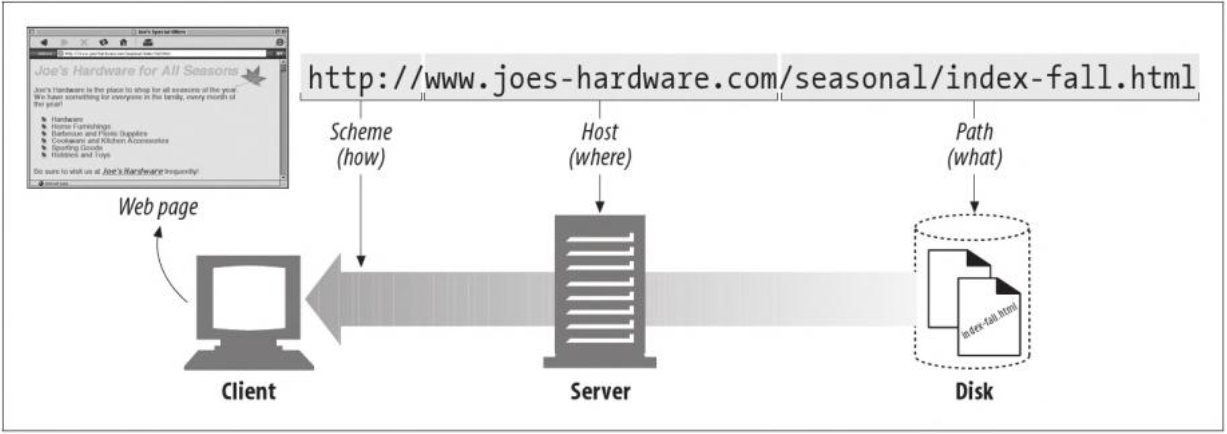
\includegraphics[width=1\textwidth]{URLDescription}
    \\
    Source: \cite[24]{gourley2002http}
\end{figure}

A transaction consists of a request (sent from client to server) and a response in which the
server answers the clients request in some way.\cite[8]{gourley2002http}
In the context of Web APIs, a request made to an API is also called "API call".\cite{StoplightAPITypes}
Figure \ref{fig:Example HTTP request and response messages} shows the structure of an 
HTTP request and response message.

\begin{figure}[H]
    \caption{Example HTTP request and response messages}
	\label{fig:Example HTTP request and response messages}
    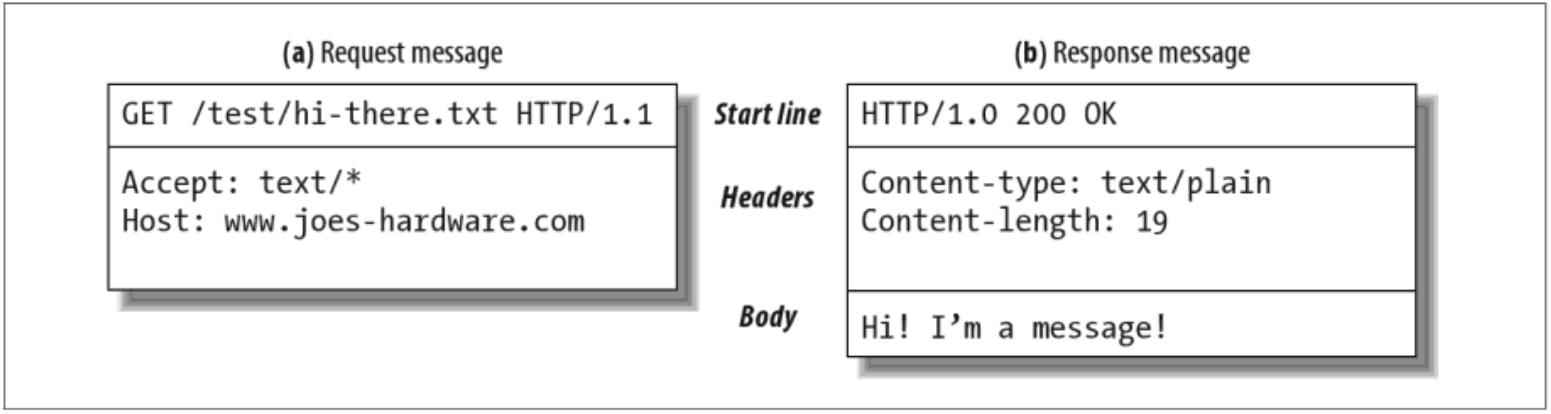
\includegraphics[width=1\textwidth]{HTTPMessageExample}
    \\
    Source: \cite[47]{gourley2002http}
\end{figure}

Every HTTP request message has a start line.
It contains a method, which tells the server what action to perform on the resource, the URL
and some protocol information.\cite[47]{gourley2002http}
After the start line, some headers are given. These contain information about the request,
e.g. what types of data the client can accept or credentials for authorization.
Some requests also contain a body to give some data to the server. \cite[52]{gourley2002http}

A response message also starts with a start line, although it does not contain a method or URL
Instead it contains protocol information and status information in the form of a numerical
status code and status text.\cite[48]{gourley2002http}
A response also contains headers and might contain a body.\cite[52]{gourley2002http}

There are many HTTP methods defined, that can be used to delete a resource, store
data on the server, get header information for a document and more.\cite[48]{gourley2002http}
In this paper, only two HTTP methods are used, GET and POST.
It is used to ask the server to send a resource to the client.
A GET request message is used to ask the server to send a resource to the client.
It does not contain a body.\cite[48]{gourley2002http}
A POST request message is used to send data to the server for processing. The data to be
processed is sent in the request body.\cite[48]{gourley2002http}

There are also many status codes defined, which tell the client the status of the transaction.
This is necessary, because the client's request can not always be fulfilled successfully
by the server.\cite[49]{gourley2002http}
The server might not be able to find the server, he might not be able to store
the data or the client might not have given the right authorization credentials to perform the
requested action. For each of these problems, there are predefined status codes.
For example, codes in the range 200-299 represent success, codes from 400-499 tell the client
that his request contained an error and 500-599 are used to inform about an error which happened on
the server.\cite[49]{gourley2002http}
Table \ref{tbl:Common status codes} shows some common status codes. There are many other
status code defined in the standard, but they are not relevant for this paper.

\begin{table}[H]
 \caption{Common status codes}
 \label{tbl:Common status codes}
\begin{tabular}{|| c | c | c ||} 
 \hline
 Status code & Reason phrase & Meaning \\ [0.5ex]
 \hline\hline
 200 & OK & Successful transaction. Any requested data is in the response body \\ [1ex]
 \hline
 401 & Unauthorized & The response needs to contain credentials to access the requested resource. \\ [1ex]
 \hline
 404 & Not Found & The server cannot find a resource for the requested URL. \\ [1ex]
 \hline
\end{tabular}
Source: \cite[50]{gourley2002http}
\end{table}

There are also many different headers defined in the HTTP standard.
Some that are important for this paper:

\begin{itemize}
    \item Authorization: Request header, which contains the credentials the client is using to authenticate.
    This might be username and password or a token.
    \item Content-Type: The datatype of the data contained in the body
\end{itemize}

\subsubsection{JSON}

Most modern APIs transmit data to the client using \ac{JSON}.
It is a text-based format able to represent structured data. \cite{MozillaJSON}
It is easy for humans to read and write JSON objects, but is also easily processed by computers.
JSON is tightly integrated in the JavaScript programming language and can be used without any parsing or serialization.\cite{OracleJSON}
This is beneficial, as JavaScript is widely used both on the client and server side of web applications. 
JSON can also be used with many other programming languages. \cite{JsonOrgIntroduction}

JSON supports only six very basic datatypes: String, Number, Boolean, Null, Object and Array.\cite{OracleJSON}
The following code snippet shows how each of the datatypes are defined in JSON.

\begin{lstlisting}[language=JavaScript]
    {
        "string": "Martin",
        "number": 200,
        "number2": 300,
        "boolean": true,
        "booleanFalse": false,
        "nullValue": null,
        "object": {
            "objectAttribute": "string",
            "objectAttribute2": "string2"
        },
        "array": [
            "entry1",
            "entry2",
            {
                "objectInArray": true
            }
        ]
    }
\end{lstlisting}

The code snippet shows, that the whole JSON object is wrapped in curly braces.
Each attribute is defined as a attribute-value-pair, where the attribute name is defined in 
double quotes, followed by a colon and the value definition. String values are defined in 
double quotes, numbers and booleans without. Objects are defined in curly braces and can
again contain any datatype.
Arrays are defined using brackets. They can contain any number of entries of any type.
Types can also be mixed within the same array.
All attributes-value-pairs or array items are seperated by commas.
Indentation and newline characters are not parsed in JSON as all syntax is given using
the characters '"{}[]:,'.\cite{JsonOrgIntroduction}

The MIME type of a JSON object is called "application/json".
An HTTP response containing JSON data will therefore always have the header
"Content-Type: application/json".\cite[Chapter 2]{richardson2008restful}

The text-based nature, good readability, simplicity and easy parsing and processing are reasons
for the wide usage of the data format. \cite{OracleJSON}
JSON is also used by the Spotify API to transfer data to the client.\cite{SpotifyWebAPI}

\subsubsection{Types of Web APIs}

As previously mentioned Web APIs are accessed through the HTTP protocol\cite{StoplightAPITypes}.
and offer a way for applications and data servers to communicate and exchange 
data over the web.\cite{Lane2019WhatIs}
They are used to power desktop, web and mobile applications. pass data between different
services, systems and devices. They make automated data access and retrieval possible
and enable the integration of internal and external systems into processes and data flows.\cite{Lane2019WhatIs}

There are different types of Web APIs.
Open or Public APIs can be used by anyone with minimal restrictions, such as logins or authentication.
They are provided by a company, government or other organization and make it possible for any developer
to access that organizations data or services.\cite{StoplightAPITypes}
Internal APIs are only used to share resources within one organization. They are meant to enable
the integration of different tools, databases and teams with each other and are not exposed to
the public.\cite{StoplightAPITypes}
Partner APIs are exposed to the public, but are only open to specific users, which might pay for
the right to use the API.
Composite APIs aggregate multiple endpoints into one to enable easy retrieval of data.
This aggregation might contain data from multiple other internal and external APIs and services.
It is used to simplify API usage and reduce server load by minimizing the number of API calls.\cite{StoplightAPITypes}

Web APIs can follow different types of architectures, which define the structure, data types
and commands used in the API. Some competing architectures are REST, RPC and SOAP. \cite{StoplightAPITypes}
As the Spotify implements a REST approach\cite{SpotifyWebAPI}, the next subsection explains the REST architecture of
Web APIs.

\subsubsection{The REST Architecture}

\ac{REST} is a set of constraints applied to modern web services, that stems from a basic set
of rules, which were defined to ensure the scalability of the web.\cite[5]{masse2011rest}
A web service, which implements REST principles is also called a "RESTful service".
Such an API consists of a set of interlinked resources called a resource model.\cite[6]{masse2011rest}

There are six basic rules to a RESTful design:\cite[2]{masse2011rest}
\begin{itemize}
    \item Client-server: The API is designed to work in a client/server architecture.\cite[3]{masse2011rest}
    \item Uniform Interface: The API needs to conform to the established standards of the web.\cite[3]{masse2011rest}
    This includes
    \begin{itemize}
        \item Identification of resources through a unique identifier, such as a URL.\cite[3]{masse2011rest}
        \item The manipulation of resources through representations.
        This means that information about the resource is only exchanged using representations.
        As an example, a set of data could be stored in a database on the server. When a client
        requests the resource, a JSON representation of the data is sent, not the actual database.
        This ensures flexibility and interoperability, as the data could also be represented using
        other models, such as XML.\cite[3]{masse2011rest}
        \item Self-discriptive messages, which means that a HTTP message should always completely
        describe the action to be performed on the server. No additional knowledge or state should
        be required to understand the message.\cite[3]{masse2011rest}
        \item Hypermedia as the engine of application state. This means that links to other
        resources can be used in a resource's representation to describe its state or the state of
        other resources.\cite[3]{masse2011rest}
    \end{itemize}
    \item Layered System: This enables the use of proxies, gateways to
    enforce security balance server load.\cite[3]{masse2011rest}
    \item Cache: The response from a web server should always include information about the
    cacheability of the response data. This ensures load reduction, availability and low latency.\cite[3]{masse2011rest}
    \item Stateless: A web server must not be required to save information about the state,
    which the client receiving the data is in. Clients should always communicate their state to
    the server so it can respond accordingly.\cite[3]{masse2011rest}
    \item Code-On-Demand: This means that servers must be able to transfer the execution of code to the client,
    e.g. in the form of client-side JavaScript.\cite[3]{masse2011rest}
\end{itemize}

All RESTful APIs should follow these rules and users of the API can expect it to handle
resources and state in this way.